% Prof. Dr. Ausberto S. Castro Vera
% UENF - CCT - LCMAT - Curso de Ci\^{e}ncia da Computa\c{c}\~{a}o
% Campos, RJ,  2022
% Disciplina: Paradigma de Desenvolvimento Orientado a Objetos
% Aluno:

\chapterimage{projeto.png} % Table of contents heading image
\chapter{Projeto do Sistema OO}
Este capítulo apresenta a arquitetura do sistema de classes, as interfaces do sistema e as tabelas de dados.

\begin{itemize}


  \item Arquitetura do Sistema que será apresentada neste capítulo mostrará o diagrama de
        componente do sistema completo e de um subsistema específico.
  \item Capturas de tela de todas as interfaces de usuário do sistema
  \item Tabelas de dados que foram utilizadas no sistema.

\end{itemize}

Um projeto orientado a objetos é um processo de criação de um conjunto de modelos de projeto orientados a objetos que são posteriormente usados por programadores para escrever e testar o novo sistema a ser desenvolvido \cite{Satzinger2012}.

\section{Arquitetura do Sistema - Classes}
\begin{itemize}
  \item Arquitetura do sistema completo (Diagrama de Componentes UML)
  \item Arquitetura de um subsistema
  \item Arquitetura de
\end{itemize}



\section{Interfaces do Usu\'{a}rio}
Toda a UI foi desenvolvida pelo autor do trabalho usando Bootstrap, um framework CSS gratuito e de código aberto voltado para desenvolvimento web front-end responsivo e mobile-first. Inclui modelos de design baseados em HTML, CSS e JavaScript para tipografia, formulários, botões, navegação e outros componentes de interface.

\begin{itemize}
  \item \textbf{ Cadastro e Login do Usuário}:
        Um dos requisitos definidos foi que o usuário deve estar cadastrado e logado para acessar o sistema.

        A imagem abaixo mostra a interface de registro do usuário onde o usuário insere nome completo, endereço de e-mail e senha. O programa verifica se o e-mail já está cadastrado. Após o preenchimento dos campos, o usuário deverá selecionar a opção “Cadastre-se” onde será redirecionado para a interface de login.
        \begin{figure}[H]
          \begin{center}
            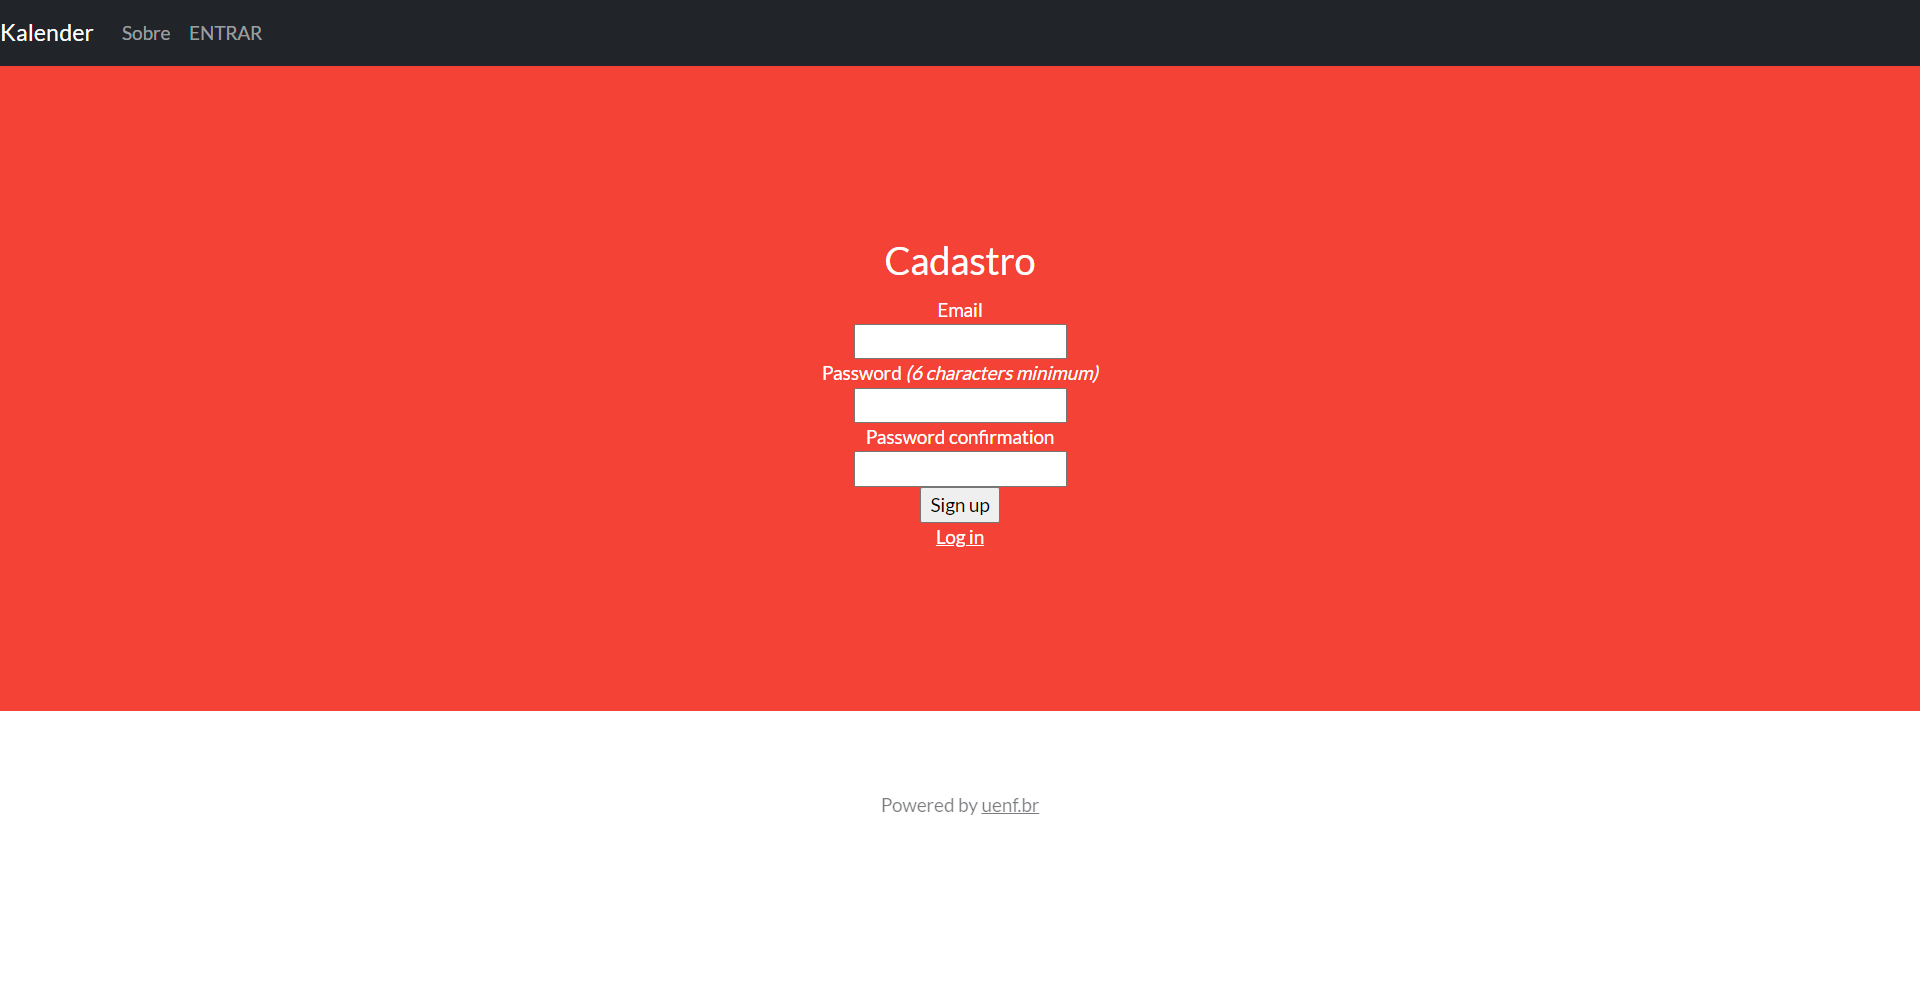
\includegraphics[width=12cm]{Pictures/interface/signup.png}
            \caption{Tela de cadastro de usuário} \label{singup}
          \end{center}
        \end{figure}
        \begin{lstlisting}[language=Ruby, caption=Interface de cadastro de usuário]
          <header class="w3-container w3-red w3-center" style="padding:128px 226px">
          <h2>Cadastro</h2>


          <%= form_for(resource, as: resource_name, url: registration_path(resource_name)) do |f| %>
            <%= render "devise/shared/error_messages", resource: resource %>

            <div class="field">
              <%= f.label :email %><br />
              <%= f.email_field :email, autofocus: true, autocomplete: "email" %>
            </div>

            <div class="field">
              <%= f.label :password %>
              <% if @minimum_password_length %>
              <em>(<%= @minimum_password_length %> characters minimum)</em>
              <% end %><br />
              <%= f.password_field :password, autocomplete: "new-password" %>
            </div>

            <div class="field">
              <%= f.label :password_confirmation %><br />
              <%= f.password_field :password_confirmation, autocomplete: "new-password" %>
            </div>

            <div class="actions">
              <%= f.submit "Sign up" %>
            </div>
          <% end %>

          <%= render "devise/shared/links" %>
          </header>
          <!-- Footer-->
          <footer class="w3-container w3-padding-64 w3-center w3-opacity">
          <!--
            <div class="w3-xlarge w3-padding-32">
              <i class="fa fa-facebook-official w3-hover-opacity"></i>
              <i class="fa fa-instagram w3-hover-opacity"></i>
              <i class="fa fa-snapchat w3-hover-opacity"></i>
              <i class="fa fa-pinterest-p w3-hover-opacity"></i>
              <i class="fa fa-twitter w3-hover-opacity"></i>
              <i class="fa fa-linkedin w3-hover-opacity" target="https://www.linkedin.com/in/arretdaniel/">uenf</i>
           </div>
          -->
           <p>Powered by <a href="https://uenf.br/portal/" target="_blank">uenf.br</a></p>
          </footer>

        \end{lstlisting}

        \begin{figure}[H]
          \begin{center}
            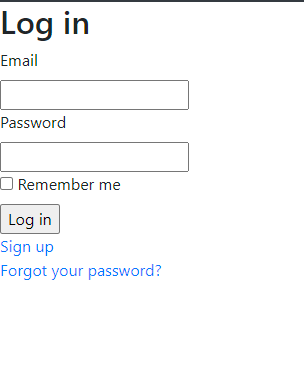
\includegraphics[width=12cm]{Pictures/interface/login.png}
            \caption{Tela de login} \label{login}
          \end{center}
        \end{figure}
        A interface de login é a interface gráfica que o usuário usa para realizar a autenticação. Onde o usuário digita o email e senha onde o programa irá verificar se o email existe e se a senha está correta.
        Caso o usuário não esteja cadastrado, basta selecionar a opção de cadastro onde será redirecionado para a interface de cadastro.


        \begin{lstlisting}[language=Ruby, caption= Código-fonte da interface de login]
      <header class="w3-container w3-red w3-center" style="padding:128px 226px">

      <h2>ENTRAR</h2>

      <%= form_for(resource, as: resource_name, url: session_path(resource_name)) do |f| %>
        <div class="field">
          <%= f.label :email %><br />
          <%= f.email_field :email, autofocus: true, autocomplete: "email" %>
        </div>

        <div class="field">
          <%= f.label :password %><br />
          <%= f.password_field :password, autocomplete: "current-password" %>
        </div>

        <% if devise_mapping.rememberable? %>
          <div class="field">
            <%= f.check_box :remember_me %>
            <%= f.label :remember_me %>
          </div>
        <% end %>

        <div class="actions">
          <%= f.submit "Log in" %>
        </div>
      <% end %>

      <%= render "devise/shared/links" %>
      </header>
      <!-- Footer-->
      <footer class="w3-container w3-padding-64 w3-center w3-opacity">
      <!--
        <div class="w3-xlarge w3-padding-32">
          <i class="fa fa-facebook-official w3-hover-opacity"></i>
          <i class="fa fa-instagram w3-hover-opacity"></i>
          <i class="fa fa-snapchat w3-hover-opacity"></i>
          <i class="fa fa-pinterest-p w3-hover-opacity"></i>
          <i class="fa fa-twitter w3-hover-opacity"></i>
          <i class="fa fa-linkedin w3-hover-opacity" target="https://www.linkedin.com/in/arretdaniel/">uenf</i>
       </div>
      -->
       <p>Powered by <a href="https://uenf.br/portal/" target="_blank">uenf.br</a></p>
      </footer>

    \end{lstlisting}


  \item \textbf{Recuperação de senha}: Caso o usuário não consiga acessar o sistema será possível solicitar recuperação da senha cadastrada, encontrará a seguinte tela, indicando que o mesmo deve fazer para prosseguir.

        \begin{figure}[H]
          \begin{center}
            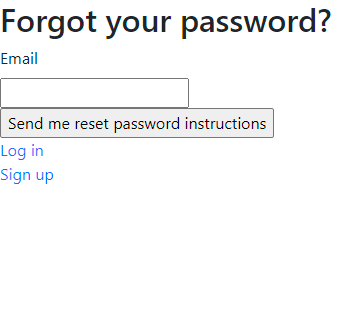
\includegraphics[width=12cm]{Pictures/interface/recuperar.png}
            \caption{Tela de recuperação de senha} \label{recuperar}
          \end{center}
        \end{figure}
        \begin{lstlisting}[language=Ruby, caption=Recuperação de senha]
          <header class="w3-container w3-red w3-center" style="padding:128px 226px">
<h2>Esqueceu sua senha?</h2>

<%= form_for(resource, as: resource_name, url: password_path(resource_name), html: { method: :post }) do |f| %>
  <%= render "devise/shared/error_messages", resource: resource %>

  <div class="field">
    <%= f.label :email %><br />
    <%= f.email_field :email, autofocus: true, autocomplete: "email" %>
  </div>

  <div class="actions">
    <%= f.submit "Envie-me instrucoes de redefinicao de senha" %>
  </div>
<% end %>

<%= render "devise/shared/links" %>
</header>
<!-- Footer-->
<footer class="w3-container w3-padding-64 w3-center w3-opacity">
<!--
  <div class="w3-xlarge w3-padding-32">
    <i class="fa fa-facebook-official w3-hover-opacity"></i>
    <i class="fa fa-instagram w3-hover-opacity"></i>
    <i class="fa fa-snapchat w3-hover-opacity"></i>
    <i class="fa fa-pinterest-p w3-hover-opacity"></i>
    <i class="fa fa-twitter w3-hover-opacity"></i>
    <i class="fa fa-linkedin w3-hover-opacity" target="https://www.linkedin.com/in/arretdaniel/">uenf</i>
 </div>
-->
 <p>Powered by <a href="https://uenf.br/portal/" target="_blank">uenf.br</a></p>
</footer>

        \end{lstlisting}

  \item \textbf{Home}: Após o login, a página inicial é exibida primeiro. Sua função é apresentar algumas informações relevantes ao usuário.
  Há um texto explicativo na tela inicial onde você pode ver onde pode se registrar para usar os recursos disponíveis para visualizar ou criar um calendário. Ao selecionar uma função, o usuário é direcionado para a tela desejada no site. A tela inicial possui uma barra que permite ao usuário alternar para outras telas do site. Em seguida, o programa retorna as partes do site que o usuário deseja combinar com o filtro. Ainda na tela inicial, o usuário pode selecionar a opção “Iniciar agora” onde será redirecionado para a interface de criação do calendário. Existem quatro opções na parte superior da tela inicial: Início (tela inicial), Entrar (para usuários que já estão registrados) e Sobre (na tela do programa). Ao abrir a tela inicial, o usuário escolhe se quer ou não manter o calendário atual.

        \begin{figure}[H]
          \begin{center}
            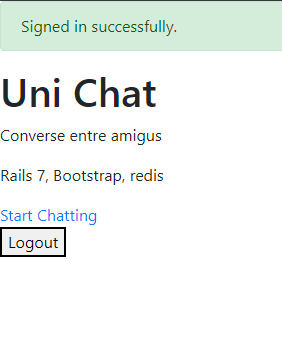
\includegraphics[width=12cm]{Pictures/interface/logged.png}
            \caption{Tela inicial do sistema (home)} \label{recuperar}
          \end{center}
        \end{figure}
        \begin{lstlisting}[language=Ruby, caption=Tela inicial do sistema (home)]

<!---->
<!---->
<!---->
<!---->
<!---->
<!--
 <h1>Kalender</h1>
  <p>Nao perca nada! Crie ja seu Kalendario</p>
-->


<!-- Header -->
<header class="w3-container w3-red w3-center" style="padding:128px 16px">
  <h1 class="w3-margin w3-jumbo">Kalender</h1>


  <% if current_user %>
  <h5> Usuario atual: <%= current_user.email.split('@')[0].capitalize %> </h5>


    <%= button_to "SAIR", destroy_user_session_path, method: :delete %>
  <% else %>
  <form action="http://127.0.0.1:3000/users/sign_up">
  <button class="w3-button w3-black w3-padding-large w3-large w3-margin-top">Comece Agora</button>
  </form>
  <% end %>
</header>

<!-- First Grid -->
<div class="w3-row-padding w3-padding-64 w3-container">
  <div class="w3-content">
    <div class="w3-twothird">
<!--
 -->
    </div>

    <div class="w3-third w3-center">
      <i class="fa fa-coffee  w3-padding-64 w3-text-red"></i>
    </div>
  </div>
</div>

<!-- Second Grid -->
<div class="w3-row-padding w3-light-grey w3-padding-64 w3-container">
  <div class="w3-content">
    <div class="w3-third w3-center">
      <i class="fa fa-calendar fa-5x w3-padding-64 w3-text-red w3-margin-right"></i>
    </div>

    <div class="w3-twothird">
      <h1>Calendario online</h1>
    </div>
  </div>
</div>

<div class="w3-container w3-black w3-center w3-opacity w3-padding-64">
    <h1 class="w3-margin w3-xlarge">Quote of the day: Wer immer wieder aufsteht hat nie wirklich verloren.</h1>
</div>

<!-- Footer-->
<footer class="w3-container w3-padding-64 w3-center w3-opacity">
<!--
  <div class="w3-xlarge w3-padding-32">
    <i class="fa fa-facebook-official w3-hover-opacity"></i>
    <i class="fa fa-instagram w3-hover-opacity"></i>
    <i class="fa fa-snapchat w3-hover-opacity"></i>
    <i class="fa fa-pinterest-p w3-hover-opacity"></i>
    <i class="fa fa-twitter w3-hover-opacity"></i>
    <i class="fa fa-linkedin w3-hover-opacity" target="https://www.linkedin.com/in/arretdaniel/">uenf</i>
 </div>
-->
 <p>Powered by <a href="https://uenf.br/portal/" target="_blank">uenf.br</a></p>
</footer>

<script>
// Used to toggle the menu on small screens when clicking on the menu button
function myFunction() {
  var x = document.getElementById("navDemo");
  if (x.className.indexOf("w3-show") == -1) {
    x.className += " w3-show";
  } else {
    x.className = x.className.replace(" w3-show", "");
  }
}
</script>



<!---->
<!---->
<!---->
<!---->
<!--

  <% if current_user %>
  <h5> Usuario atual: <%= current_user.email.split('@')[0].capitalize %> </h5>
    <%= link_to "Crie ja seu Calendario", lands_landpage_path %>

    <form action="http://[::1]:3000/lands/landpage">
    <button class="button2 button1">VER KALENDER</button>
    </form>

    <%= button_to "SAIR", destroy_user_session_path, method: :delete %>
  <% else %>
    <%= link_to "CADASTRO", new_user_registration_path %>
    <%= link_to "ENTRAR", new_user_session_path %>
  <% end %>
-->

        \end{lstlisting}

        A tela da lista de calendários destina-se a usuários que desejam visualizar suas tarefas de maneira tradicional em vez de usar um calendário completo. Na tela da lista de calendários, o usuário pode selecionar uma tarefa para visualizar os detalhes, que serão direcionados para a tela de detalhes da atividade. Assim como na tela inicial com a tarefa, a tela da lista de atividades possui uma barra que permite ao usuário ir para outras partes do site, Home (tela inicial), Login (para usuários já cadastrados) e Sobre (no menu do programa). Em seguida, o programa retorna as atividades que correspondem ao filtro.
        \begin{figure}[H]
          \begin{center}
            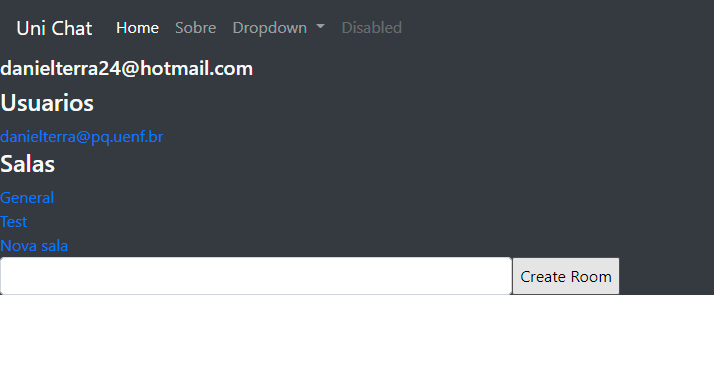
\includegraphics[width=12cm]{Pictures/interface/chat1.png}
            \caption{Tela inicial (Calendario)} \label{chat1}
          \end{center}
        \end{figure}
        \begin{lstlisting}[language=Ruby, caption=Ruby Controller]
          <header class="w3-container w3-red w3-center" style="padding:128px 226px">
<!--
<div class="container mt-5 text-center">
   -->
  <h1>Kalender</h1>
  <p>Seja Bem-vindu:</p>

  <h5> <%= current_user.email.split('@')[0].capitalize %> </h5>


<form action="http://[::1]:3000/consultations/new">
<button class="button1 button1">Criar nova atividade!</button>
</form>

  <%= month_calendar(events: @consultations) do |date, consultations| %>
    <div class="day">
      <%= date %>
    </div>
    <% consultations.each do |consultation| %>
      <div class="card-header">
        <h5 class="card-title">
          <%= link_to consultation.title, consultation %>
        </h5>
      </div>
      <div class="card-body">
        <p class="card-text">
          <%= consultation.description %>
        </p>
      </div>
      <div class="card-footer">
        <p class="card-text">
          From: <%= consultation.start_time.strftime('%A, %B %d, %Y at %I:%M %p') %>
        </p>
        <p class="card-text">
          To: <%= consultation.end_time.strftime('%A, %B %d, %Y at %I:%M %p') %>
        </p>
      </div>
    <% end %>
  <% end %>
</div>
</header>
<!-- Footer-->
<footer class="w3-container w3-padding-64 w3-center w3-opacity">
<!--
  <div class="w3-xlarge w3-padding-32">
    <i class="fa fa-facebook-official w3-hover-opacity"></i>
    <i class="fa fa-instagram w3-hover-opacity"></i>
    <i class="fa fa-snapchat w3-hover-opacity"></i>
    <i class="fa fa-pinterest-p w3-hover-opacity"></i>
    <i class="fa fa-twitter w3-hover-opacity"></i>
    <i class="fa fa-linkedin w3-hover-opacity" target="https://www.linkedin.com/in/arretdaniel/">uenf</i>
 </div>
-->
 <p>Powered by <a href="https://uenf.br/portal/" target="_blank">uenf.br</a></p>
</footer>

        \end{lstlisting}

        \item \textbf{Sobre}: As informações (Sobre) sobre o aplicativo são exibidas na tela, por exemplo: Autores, instituição e descrição da candidatura.

              \begin{figure}[H]
                \begin{center}
                  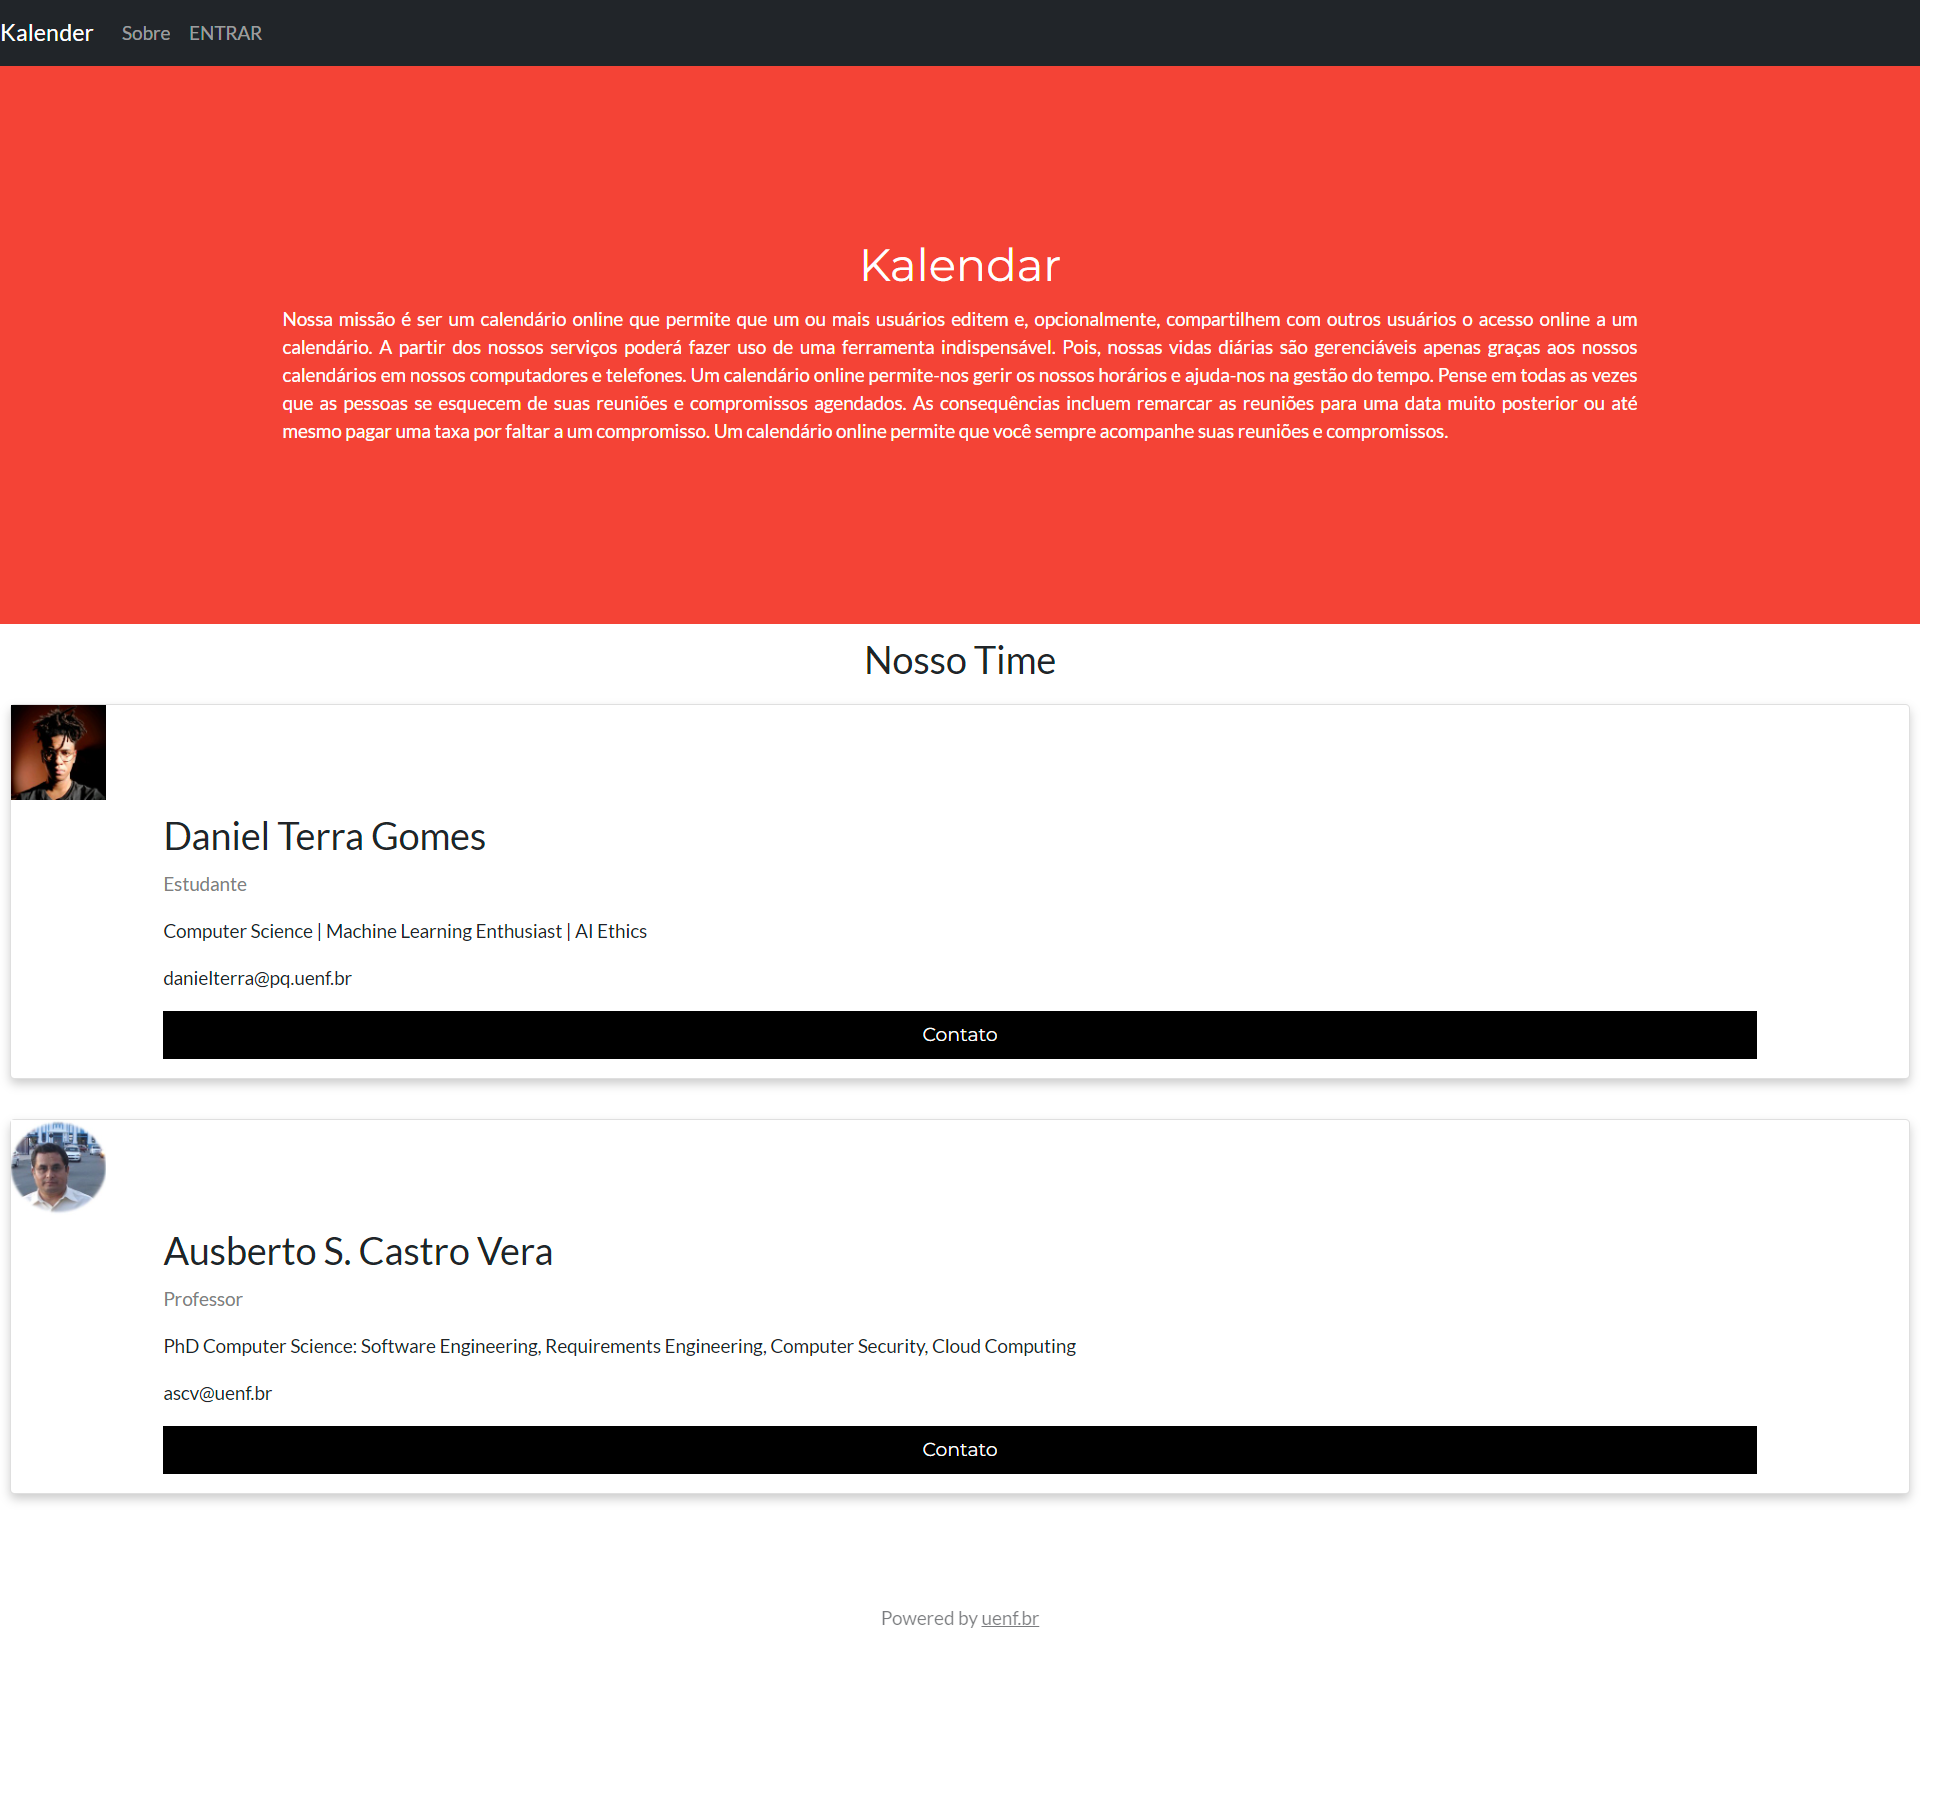
\includegraphics[width=12cm]{Pictures/interface/sobre.png}
                  \caption{Interface de sobre} \label{sobre}
                \end{center}
              \end{figure}
              \begin{lstlisting}[language=Ruby, caption=Tela inicial do sistema (home)]

        \begin{lstlisting}[language=Ruby, caption=About Us]
          <div class="about-section">
            <h1>Kalendar</h1>

            <p class="div">Nossa missao e ser um calendario online que permite que um ou mais usuarios editem e, opcionalmente, compartilhem com outros usuarios o acesso online a um calendario.

          A partir dos nossos servicos podera fazer uso de uma ferramenta indispensavel. Pois, nossas vidas diarias sao gerenciaveis apenas gracas aos nossos calendarios em nossos computadores e telefones. Um calendario online permite-nos gerir os nossos horarios e ajuda-nos na gestao do tempo. Pense em todas as vezes que as pessoas se esquecem de suas reunioes e compromissos agendados. As consequencias incluem remarcar as reunioes para uma data muito posterior ou ate mesmo pagar uma taxa por faltar a um compromisso. Um calendario online permite que voce sempre acompanhe suas reunioes e compromissos.</p>

          </div>

          <h2 style="text-align:center">Nosso Time</h2>
          <div class="row">
            <div class="column">
              <div class="card">
                <img src="https://media-exp1.licdn.com/dms/image/C4E03AQFXwSHsXB5A-w/profile-displayphoto-shrink_200_200/0/1653855378664?e=1671062400&v=beta&t=JnZi5-8DhyHSwJWl68lXvud1KkoxXQDeGJyuVxGWdRY" alt="Daniel" style="width:5%">
                <div class="container">
                  <h2>Daniel Terra Gomes</h2>
                  <p class="title">Estudante</p>
                  <p>Computer Science | Machine Learning Enthusiast | AI Ethics</p>
                  <p>danielterra@pq.uenf.br</p>
                  <p><button class="button">Contato</button></p>
                </div>
              </div>
            </div>

            <div class="column">
              <div class="card">
                <img src="https://media-exp1.licdn.com/dms/image/C5603AQHKXoHRT58ayQ/profile-displayphoto-shrink_200_200/0/1516814846280?e=1671062400&v=beta&t=cic_dbtWwgtjWRRnokSRsCxRugh6w52FOZYAksyRxEs" alt="Ausberto" style="width:5%">
                <div class="container">
                  <h2>Ausberto S. Castro Vera</h2>
                  <p class="title">Professor</p>
                  <p>PhD Computer Science: Software Engineering, Requirements Engineering, Computer Security, Cloud Computing</p>
                  <p>ascv@uenf.br</p>
                  <p><button class="button">Contato</button></p>
                </div>
              </div>
            </div>


          </div>

          \end{lstlisting}
\end{itemize}


\section{Tabelas de Dados}
O sistema gerenciador de Banco de Dados SQLite3 foi utilizado para o desenvolvimento do calendário. SQLite é uma biblioteca de domínio público que contém um sistema de banco de dados relacional. SQLite é usado em telefones celulares, em navegadores, Skype e muitos outros aplicativos. É o sistema de banco de dados mais difundido e usado no mundo, implementando um mecanismo de banco de dados SQL pequeno, rápido, independente, de alta confiabilidade e com todos os recursos.

Foram criados os seguintes:

\begin{lstlisting}[language=Ruby, caption=schema]

  ActiveRecord::Schema[7.0].define(version: 2022_10_14_155028) do
    create_table "consultations", force: :cascade do |t|
      t.string "title"
      t.text "description"
      t.datetime "start_time"
      t.datetime "end_time"
      t.datetime "created_at", null: false
      t.datetime "updated_at", null: false
    end

    create_table "users", force: :cascade do |t|
      t.string "email", default: "", null: false
      t.string "encrypted_password", default: "", null: false
      t.string "reset_password_token"
      t.datetime "reset_password_sent_at"
      t.datetime "remember_created_at"
      t.datetime "created_at", null: false
      t.datetime "updated_at", null: false
      t.boolean "admin", default: false
      t.index ["email"], name: "index_users_on_email", unique: true
      t.index ["reset_password_token"], name: "index_users_on_reset_password_token", unique: true
    end

  end

  \end{lstlisting}
\begin{lstlisting}[language=Ruby, caption=CreateConsultations]

  class CreateConsultations < ActiveRecord::Migration[7.0]
    def change
      create_table :consultations do |t|
        t.string :title
        t.text :description
        t.datetime :start_time
        t.datetime :end_time

        t.timestamps
      end
    end
  end



  \end{lstlisting}

  \begin{lstlisting}[language=Ruby, caption=AddAdminToUser]
  class AddAdminToUser < ActiveRecord::Migration[7.0]
    def change
      add_column :users, :admin, :boolean, default: false
    end
  end





  \end{lstlisting}

  \begin{lstlisting}[language=Ruby, caption=DeviseCreateUsers]

  # frozen_string_literal: true

  class DeviseCreateUsers < ActiveRecord::Migration[7.0]
    def change
      create_table :users do |t|
        ## Database authenticatable
        t.string :email,              null: false, default: ""
        t.string :encrypted_password, null: false, default: ""

        ## Recoverable
        t.string   :reset_password_token
        t.datetime :reset_password_sent_at

        ## Rememberable
        t.datetime :remember_created_at

        ## Trackable
        # t.integer  :sign_in_count, default: 0, null: false
        # t.datetime :current_sign_in_at
        # t.datetime :last_sign_in_at
        # t.string   :current_sign_in_ip
        # t.string   :last_sign_in_ip

        ## Confirmable
        # t.string   :confirmation_token
        # t.datetime :confirmed_at
        # t.datetime :confirmation_sent_at
        # t.string   :unconfirmed_email # Only if using reconfirmable

        ## Lockable
        # t.integer  :failed_attempts, default: 0, null: false # Only if lock strategy is :failed_attempts
        # t.string   :unlock_token # Only if unlock strategy is :email or :both
        # t.datetime :locked_at


        t.timestamps null: false
      end

      add_index :users, :email,                unique: true
      add_index :users, :reset_password_token, unique: true
      # add_index :users, :confirmation_token,   unique: true
      # add_index :users, :unlock_token,         unique: true
    end
  end





  \end{lstlisting}
